\documentclass[a4paper]{article}

\usepackage{color}
\usepackage{url}
\usepackage[T2A]{fontenc}
\usepackage[utf8]{inputenc}
\usepackage{graphicx}

\usepackage[english,serbian]{babel}

\usepackage[unicode]{hyperref}
\hypersetup{colorlinks,citecolor=green,filecolor=green,linkcolor=blue,urlcolor=blue}


\begin{document}

\title{Propisi i standardi verifikacije softvera u automobilskoj industriji\\ \small{Seminarski rad u okviru kursa\\Metodologija stručnog i naučnog rada\\ Matematički fakultet}}

\author{
Andrea Pilipović\\ andrea.pilipovic@yahoo.com\\ 
Vojkan Cvijović\\ vojkancvijovic@gmail.com\\ 
Strahinja Stanojević\\ strahinjastanojevic@rocketmail.com\\ 
Saša Cvetković\\ sasa.cvetkovic@yahoo.com}

\date{18.~april 2018.}
\maketitle

\tableofcontents

\newpage

\section{Uvod}
\label{sec:uvod}

U velikoj većini različitih industrija se koriste embeded sistemi kako bi se podigla pouzdanost različitih sistema. Obično su to sistemi koji zahtevaju visoku pouzdanost i bezbednost. Sistemi od kojih mogu zavisiti i ljudski životi. Jedna od takvih industrija je i automobilska industrija. Potreba za korišćenjem softvera u ovoj industriji kao i sama njihova upotreba je značajno porasla u poslednjoj deceniji \cite{ref1} \cite{ref2}. Većina funkcionalnosti u modernim automobilima, posebno one funkcije koje su vezane za bezbednost, kao što su automatske kočnice ili automatski asistenti pri vožnji \cite{ref3}, kontrolišu se pomoću softvera \cite{ref4}. Predviđa se da će oko 90\% automobila u budućnosti biti voženo softverski, bez ljudske pomoći \cite{ref2}.


\section{Softver u automobilskoj industriji}
\label{sec:softer}

Automobilska industrija je tradicionalno pretežno bazirana na konceptima mašinskog inženjerstva \cite{ref5}\cite{ref6}. Baš kao i neke druge industrije koje su tradicionalno ne-softverske, kao što su avionska, odbrambena ili raketna, i automobilska industrija biva pogodjena softverskom revolucijom. Sve veći broj, kako kritičnih tako i ne kritičnih, funkcionalnosti automobila počinje da bude kontrolisano pomoću softvera. Stoga je razumevanje softvera koji se koriste u automobilskoj industriji sve važnije, i mnogo se više pažnje pridaje nego pre par decenija. Broj (eng. Broy) u \cite{ref6} opisuje softver u ovoj industriji na sledeći način:
\bigbreak
\textit{veličina}: Za 40 (od 1976. \cite{ref7}) godina broj linija koda u automobilskoj industriji se povećao sa nula na nekoliko miliona.
\bigbreak
\textit{uloga}: Funckije u vozilima, kako kritične kao što su kočioni sistem, tako i ne kritične (radio, klima i slično) danas se kontrolišu pomoću softvera. 
\bigbreak
\textit{interakcija i rasprostranjenost}: U automobilima postoje ECU sistemi, koji su u suštini mikrokontroleri koji odgovaraju softverskim komponentama \cite{ref38}. ECU sistemi rade zajedno kako bi izvršili potrebnu funkciju automobila. Te funkcije mogu biti veoma raznorodne, kao na primer kontrolisanje motora, vazdušnih jastuka ili prikaz nivoa goriva \cite{ref8}. U prošlosti, svaki ECU sistem je izvršavao posebnu funkcionalnost. Zbog toga su softverski mogle da se izvršavaju samo funkcije koje je mogao da izvršava jedan ECU sistem. Ranih devedesetih, ECU sistemi su bili povezani lokalnom mrežom CAN (eng. Control Area Network) pomoću koje su mogli da komuniciraju i dele informacije. Ovo je dovelo do funkcija koje su bile kompleksnije i bilo je potrebno da ih zajedno izvršava više ECU sistema. U kasnim devedesetim, funkcije su bile toliko kompleksne da je bilo potrebno da postoji komunikacija izmedju više CAN mreža. Danas, sem komunikacije medju CAN mrežama unutar samog automobila, vrši se i njihova komunikacija sa spoljašnjim okruženjem pomoću radio veza \cite{ref2}.
\bigbreak
Do sada navedene karakteristike su samo dokaz da je upotreba softvera jako velika u automobilskoj industriji danas. Takođe, pokazuje da je softver neizostavni deo današnjih automobila. Bojl dalje u \cite{ref7} opisuje karakteristike softvera u automobilskoj industriji. Naredne stavke govore o kompleksnosti samog softvera.
\bigbreak
\textit{heterogenost podsistema}: Pri izradi softvera za automobil koristi se modularnost, kao i uopste pri proizvodnji automobila. Tako se rade softveri za kontrolisanje različitih sistema, kočnica, menjača, motora, a zatim se oni pojedinačno testiraju. Nakon uspešnog testiranja, sistemi se objedinjavaju u jedna jedinstven sistem vozila. 
\bigbreak
\textit{proivođači originalne opreme} (eng. Original Equipment Manufacturer (OEM)): Proces integracije heterogenih sistema je sam po sebi zahtevan, međutim ovaj zadatak je daleko kompleksniji. To je tako zbog činjenice da veliki broj sistema za vozila dolazi od različitih proizvođača. Kasnije je zadatak automobilskih kompanija da ove sisteme i softvere dobijene od različitih proizvođača objedine i integrišu.
\bigbreak
\textit{visoko konfigurabilni softver}: Softveri u automobilskoj industriji su visoko konfigurabilni, s obzirom na to da postoji veliki broj različitih funkcija koje automobil obavlja. S toga, veliki broj različitih varijanti vozila može biti proizveden od modularnih delova. Na primer, autori \cite{ref7} navode primer vozila sa 80 različitih softverskih jedinica, gde jednostavan izbor da li se funkcionalnost svakog od njih uključuje ili ne vodi do (2 na 80) mogućnosti. Iz ovoga se zaključuje da je moguće napraviti više varijanti vozila koji se razlikuju po funkcionalnostima koje su uključene i dobijene su kombinovanjem različitih softverskih jedinica.
\bigbreak
\section{Značaj verifikacije u automobilskoj industriji}
\label{sec:znacajverifkacije}

Verifikiacija softvera, i testiranje kao jedna od oblasti verifikacije je doživela ekspanziju poslednjih godina, posebno u osetljivim oblastima, kao što su avionska, raketna, automobilska i slične. Ipak, što se same automobilske industrije tiče, ne postoji previše studija koje se fokusiraju na testiranje i verifikaciju na višim nivoima, pri integraciji pojedinačnih komponenti. Međutim, postoji potreba za fokusom i akademskih i industrijskih istraživača u ovoj oblasti.
\bigbreak
S obzirom na sve veći broj funkcionalnosti koje pružaju današnji automobili, softveri bivaju sve kompleksniji. Jedan od glavnih zadataka u automobilskoj industriji je dizajnirati efektivne i efikasne procese izrade i testiranja softvera \cite{ref9}. S obzirom na sve kompleksnije i veće softvere sa sve većim brojem mogućnosti i funkcionalnosti, njihova verifikacija i testiranje postaje dosta kompleksan zadatak \cite{ref10}. Neotkrivene greške u softveru u ovoj industriji mogu imati jako ozbiljne posledice. Može doći do saobraćajnih nesreća, povreda, pa čak i do gubitka ljudskih života. Zbog ovoga je izuzetno važno izvršiti detaljno testiranje svih delova softvera. Samo jedna greška može dovesti do katastrofalnih posledica \cite{ref11}. Upravo iz ovog razloga, oko 50\% od ukupnog vemena koje se utroši na tehničke aktivnosti (vezane za izradu softverskog dela) u razvoju vozila se potroši na testiranje samog softvera \cite{ref12}.


\bigbreak
Neki od primera kada su greške u softveru mogle da dovedu do katastrofalnih posledica:
\bigbreak
Proizvodjač automobila Tojota (eng. Toyota) je 2009. i 2010. godine imao prijave vozila koja su ubrzavala sama od sebe bez ikakvog razloga. Ispostavilo se da je problem bio u softveru koji je kontrolisao ubrzavanje vozila. Isti proizvođač je imao jos prijava. Nakon prijave jos jednog problema na nekoliko vozila kompanija je odlučila da napravi novi hibridni softver. Drugi problem je bio vezan za kočioni sistem, što je moglo rezultovati čak i ljudskim žrtvama. 
\bigbreak
14. februara 2016. godine, Guglov (eng. Google) samovozeći automobil (self-driving car) je izazvao nesreću na semaforu. Kompanija je priznala da je problem bio greška softvera u predviđanju kretnje autobusa, kao i u odluci šta sam automobil treba da uradi, odnosno kuda da ide. Nakon otvranja zelenog svetla za automobil, on je uspešno detektovao autobus, međutim pretpostavka koju je napravio je da će autobus usporiti, tako da je krenuo dalje. Nesreća nije bila velikih razmera.

\section{Izazovi u verifikaciji softvera u automobilskoj industriji}
\label{sec:izazovi}

U ovom delu dajemo kratak pregled izazova koji se mogu sresti u verifikaciji softvera u automobilskoj industriji \cite{ref13}\cite{ref14}\cite{ref15}.
\bigbreak
\textit{merenje napora}: Poteskoće u određivanju važnosti testiranja na različitim nivoima \cite{ref14}.
\bigbreak
\textit{znanje osoblja}: Različita mišljenja različito stručnih ljudi \cite{ref14}.
\bigbreak
\textit{distribuirane funkcionalnosti}: Visoka kompleksnost testova usled distribuiranosti softvera \cite{ref14}.
\bigbreak
\textit{metrika pokrivenosti}: Nedostatak podrške za merenje testova \cite{ref14}. 
\bigbreak
\textit{različite varijante}: Kombinatorna eksplozija testiranja zbog visokog stepena prilagođavanja \cite{ref14}.
\bigbreak
\textit{zahtevi i mogućnost praćenja}: Problemi vezani za zahteve kao što su nedostatak jasnih zahteva za testove visokog nivoa i nedostatak praćenja napretka kao prepreka za verifikaciju \cite{ref13}.
\bigbreak
\textit{proces testiranja}: Odsustvo jedinstvenog procesa testiranja \cite{ref13}.
\bigbreak
\textit{alati za verifikaciju}: Nedostatak adekvatnih alata i tehnika za verifikaciju \cite{ref13}.
\bigbreak
\textit{testiranje i praćenje nedostataka}: Visoka cena popravljanja nedostataka kao i neotkrivenih nedostataka \cite{ref13}.
\bigbreak
\textit{dokumentacija}: Nedostatak odgovarajuće i ažurne dokumentacije \cite{ref13}.
\bigbreak
\textit{dokumentacija}: Preklapanje testova na različitim nivoima testiranja dovodi do gubitka vremena i resursa \cite{ref15}.


\section{Efikasno testiranje u automobilskoj industriji}
\label{sec:efikasno}

Softverski sistemi postaju sve više kompleksniji i sve više se izvršavaju u okruženjima gde je bezbednost od izuzetne važnosti, na primer sistemi za pomoć pri upravljanju vozilom. Stoga kvalitet softvera je vrlo bitna stavka kod automobilskih softverskih sistema. Testiranje softvera je jedna od najbitnijih stavki prilikom razvoja softvera za automobile. Bilo kakve greške na softveru koje se ne otkriju prilikom testiranja, mogu da izazovu ogromne finansijske probleme i čak da rizikuju ljudske živote.
\bigbreak

Proces testiranja softvera je, prema Spillner i Linz, podeljen u pet faza, kao što je prikazano u figuri 1. Počinje se sa fazom planiranja. Koncept testa i plan testa su definisani u ovoj fazi. Resursi moraju biti raspoređeni i ciljevi svakog testa moraju biti definisani. Posle početnog planiranja, sledi faza analize i dizajna. U toj fazi svi slučajevi se opisuju na apstraktan način i definišu se prema specifikaciji softvera. Nakon toga svi test slučajevi se moraju implementirati, dalje se vrši odabir testova, pokreću se na sistemu za testiranje, ručno ili automatski. Kada se izvršavanje testova završi, rezultati se sakupljaju i dokumentuju za dalju analizu. Osoba odgovorna za projekat mora da odluči koji su dalji testovi neophodni. Ovo se može utvrditi na primer, posmatranjem učestalosti dešavanja kvarova i popravki na sistemu. Novi testovi se izvršavaju ako je to potrebno.

\bigbreak

Generalno testiranje je u velikoj meri ograničeno resursima stoga je cilj da testiranje bude efikasnije i da u isto vreme bude i efektivnije. U automobilskom softverskom testiranju, postoje posebni izazovi. Prvo, u automobilskoj industriji postoji posebna veza između proizvođača, dobavljača i testera. Pošto su softverske komponente obično razvijene od strane dobavljača i testirane lokalno, integraciju obavlja proizvođač ili je izvršena od strane drugog dobavljača. Usled ugovorenih ograničenja, izvorni kod nije dostupan za integraciono i sistemsko testiranje. To dovodi do metode testiranja crnom kutijom gde je testiranje zasnovano na specifikaciji sistema. Drugo, proizvodi testiranja su često naznačeni u prirodnom jeziku \cite{ref20}. Ovo otežava pravljenje pretpostavki u vezi progresa testiranja i pokrivenosti sistema na kome se testira i automatizacije izbora test slučaja i njihovog izvršavanja. Treće, u većini slučajeva, svi naznačeni test slučajevi ne mogu biti izvršeni zbog ograničenja resursa. Stoga, mora biti izabran podskup test slucajeva. Ovo je veoma kritičan zadatak, pošto nije jednostavno da se izabere pravi test slučaj, koji će verovatno uočiti grešku. U metodi testiranja crnom kutijom, koja je greška za automobilske softvere i sisteme, izvorni kod nije dostupan. To dovodi do nedostatka popularne pokrivenosti koda. Umesto toga, druge heuristike moraju da budu uvedene u automobilsko područije za izbor test slučajeva. Četvrto, u automobilskom softverskom razvoju, dosta pod-procesa od celokupnog procesa testiranja se izvršavaju ručno. Automatizacija testiranja procesa, uključujući izbor i prioritet test slučaja, je željeni cilj, pošto može da smanji napor testiranja u poređenju na ručno izvršenje\cite{ref16}.
\bigbreak

Kako bi automobilsko softversko testiranje napravili više efikasnim, u ovom papiru, predstavićemo šest različitih izazova testiranja i prema rešenjima u automobilskom razvoju softvera uzimajući u obzir određena ograničenja i izazove u ovom područiju. Ovaj pristup pokriva test slučajeve u prirodnom jeziku, automobilizaciju izbora i prioritizacija test slučaja. Prikazaćemo zadati koncept pomoću primera, Body Comfort System \cite{ref17}.
\bigbreak
 
\section{Analiza i dizajn}
\label{sec:analiza}

U ovoj fazi glavni zadatak je kreiranje slučajeva za testiranje, kako to predstavlja odnos samog procesa testiranja. Ova faza je važna za bilo koju formu testiranja, kako se u njoj definiše koje informacije su dostupne i kako im pristupiti prilikom testiranja. Greške iz ove faze mogu biti jako skupe u narednim fazama, na primer, nedovoljan opis testa, redudanran test slučaj. Što se pre otkriju takve greške, to ih je lakše rešiti.
U daljem teksu se opisuju dva načina na koji mogu da se unaprede testovi u ovoj fazi testiranja. Prvo se opisuje specifikacija za opis test slučajeva, dalje se predlaže koncept za uklanjanje redudantnih test slučajeva.

\subsection{Specifikacija test slučajeva koji se testiraju metodom crne kutije}
\label{subsec:spectestslucaj}


U fazi analize, test slučajevi su neretko formulisani u nekom govornom jeziku. Uobičajno je da se test slučaj sastoji od preduslova, akcije i očekivanog rezultata. Akcije su podeljene na veći broj koraka koji tester mora da izvrši. Test slučajevi su obično povezani određenim uslovnostima, što je obično zadato u specifikaciji tog test slučaja. I preduslovi i koraci test slučaja se uglavnom čuvaju u određenim alatima poput, HP Quality Center, IBM DOORS. Takvi alati omogućavaju praćenje test slučajeva, njihovih razlika i preduslova. Cilj u testiranju metodom crne kutije je da se postigne zacrtana pokrivenost zahteva testovima. Na primer, test slučaj za zaštitu prstiju prilikom zatvaranja prozora, može biti opisan u govornom jeziku. Specifikacija ove funkcionalnosti se sastoji od, u slučaju da je omogućena zaštita prstiju, detektuje se objekat, prsti, prilikom zatvaranja prozora i zatvaranje prozora se prekida kako ne bi došlo do povrede. Test slučaj ove funkcionalnosti moze se definisati na dva različita načina kao što je pokazano na slici \ref{fig:slika1}. Najčešći problem prilikom definisanja test slučaja je sam opis test slučaja. Kako se govorni jezik koristi za opis, od testera zavisi kako će test slučaj biti opisan.

\bigbreak
\begin{figure}[h!]
\begin{center}
\includegraphics[scale=0.5]{slika1.jpg}
\end{center}
\caption{Test slučaj otiska prsta}
\label{fig:slika1}
\end{figure}
\bigbreak

Na primer, u prikazanim testovima na slici \ref{fig:slika1}, u opisu jednog testa se nalaze pune rečenice dok kod drugog se nalaze samo stavke. Skraćenice mogu da izazovu probleme, moraju se definisati. U suprotnom test slučaj postaje nedovoljano jasan drugim saradnicima. Postoje mnogi slučajevi gde definicije test slučajeva mogu da se razlikuju ali da se odnose na istu funkcionalnost.
\bigbreak

U slučaju da se test slučajevi analiziraju, sledeći aspekti se moraju razmotriti: da li je neka komponenta ili funkcionalnost već pokrivena više nego ostale funkcionalnosti, da li postoje redudantnosti među testovima, da li su neki test slučajevi previše komplikovani, da li određeni testovi mogu da se iskombinuju. Ako bi se koristio alat za analiziranje test slučajeva, moglo bi da dođe do problema u slučaju da opisi testova nisu konzistentni. Ovo zahteva da se testovi dizajniraju korišćenjem određenog vokabulara, da sadrže samo određene fraze i unapred definisane strukture. Na primer, potrebno je da test dizajner piše PowerWindow i definiše redom preduslove, akcije i očekivani rezultat. Može biti definisano, koliko najviše koraka može jedan test slučaj da sadrži. Potrebno je definisati sve neophodne prekidače, polja, parametre i način kako se oni referišu u opisu test slučaja. Ovo dovodi do uniformisanja test slučajeva. Na kraju, test slučajevi moraju biti podržani od strane korišćenih alata. Ti alati mogu da predlože dizajneru testova, koje parametre da refereiše, gde da ih piše...
\bigbreak

\subsection{Uklanjanje redudansi}
\label{subsec:redundansi}

Izazov je rukovati velikim skupom testova prilikom razvoja softvera. Broj test slučajeva se uvećava vremenom, kako novi projekti u kompanije se često baziraju na prethodnim verzijama softvera i koriste proizvode koji su kreirani u drugim projektima \cite{ref18}. Takvi proizvodi mogu biti uslovni, softverske komponente, test slučajevi. Ali ponovno korišćenje može da dovede do redudantnosti među proizvodima. Na primer, razvija se nova verzija sistema, za novi model. Prethodna verzija je imala nekoliko hiljada testova, od kojih većina može biti ponovo korišćena. Testovi se kopiraju u novi projekat ali potrebno je testirati nove funkcionalnosti. Ovo dovodi do toga da se dizajniraju novi testovi. Kako tester ne može da proveri opis i cilj hiljadu starih testova, moguće je da pojedini novi testovi su već pokriveni starim testovima. Ovo može lako da se dogodi u slučaju da više od jednog dizajnera radi na istoj funkcionalnosti.
\bigbreak

Redudantnost može da dovede do velike neefikasnosti testiranja kako se jedan isti test slučaj testira nekoliko puta bez promene rezultata. Jedno rešenje jeste da se ne koriste gotovi proizvodi. To bi značilo da testeri moraju da napišu svaki test slučaj od početka. Pa sledi da ovo nije bas efikasan način, zbog velikog broja testova. Potreban je pametniji pristup, pristup koji može da detektuje i otkloni redudantnosti dok u isto vreme omogućava veliku iskorišćenost gotovih proizvoda. Testovi se porede kako bi se našli isti delovi. Ovo zahteva da su test slučajevi napisani na taj način da mogu da se porede. Nakon procesiranja specifikacije test slučaja, redudantni test slučajevi mogu biti obeleženi ili u potpunosti uklonjeni. Kada se piše novi test slučaj, test dizajner može biti direktno upozoren ako je novi test sličan postojećem. 
\bigbreak

\section{Implementacija i egzekucija}
\label{sec:implementegzek}

Kada su svi testovi opisani, potrebno je da budu i izvršeni. Moguće je da se za testove visokog nivoa moraju implementirati i neke dodatne test skripte. Iako su test slučajevi sistematično opisani i bez redudantnosti, mora se pronaći balans između potencijalno velikog broja dizajniranih testova i veoma ograničenih resursa za testiranje. Glavni izazovi su selekcija test slučajeva koji će biti izvršeni i njihovo sortiranje. Prioritizacija test slučajeva \cite{ref21}\cite{ref19} je neophodna i uglavnom ne mogu svi odabrani testovi biti izvršeni zato što neki testovi moraju biti ručno izvršeni. U proiritizaciji testova, važniji testovi se izvršavaju prvo. Zbog toga se neki ciljevi testiranja postižu ranije, što je poželjno, pogotovu ako ne mogu svi odabrani testovi biti testirani. U automobilskoj industriji odabir testova i njihova prioritizacija predstavlja izazov s obzirom da je izvorni kod sistema koji se testira nepoznat. Takvo testiranje metodom crne kutije omogućava vrlo ograničene informacije, poput pokrivenosti koda, za razliku od tehnika metode bele kutije.
\bigbreak

\subsection{Efektivna selekcija testnih slučajeva i prioritizacija u testovima crne kutije}
\label{subsec:efektivnaselekcija}

Prvo pitanje, na koje treba dati odgovor, jeste šta zapravo predstavlja jedan dobar testni slučaj. Ovo pitanje nas dovodi do činjenice da je neophodno uložiti veliki napor pri izboru slučajeva testiranja. Kaner \cite{ref22} je istraživao ovo pitanje i opisao kvalitet testnog slučaja koristeći nekoliko faktora. U opštem testiranju, dobar testni slučaj se može definisati prema nekoliko različitih kriterijuma. Neki od mogućih primera su slučajevi kada test ima veliku verovatnoću da pronađe grešku, test testira funkcije koje se verovatno koriste u stvarnosti itd. Zbog toga, za odabir test slučajeva je važno odabrati one testne slučajeve koji odgovaraju trenutnom testnom cilju.
\bigbreak

Pretpostavljajući korišćenje slučajeva testiranja na visokom nivou u slučaju testiranja crne kutije, kreiranje test slučajeva je obično ručni zadatak, koji podrazumeva veliku količinu stručnog znanja i iskustva u vezi sa sistemom koji se testira. To dovodi do dva glavna problema. Prvo, poznavanje kreiranih testova slučajeva i njihovog dizajna se često gubi kada osoba napusti projekat ili kompaniju. Baš zbog te činjenice, druge osobe ne mogu da ponove testiranje. Zadatak kreiranja novih testnih slučajeva je proces koji može dugo trajati zbog potrebe za razvijanjem potrebne veštine za kreiranje "dobrih" testnih slučajeva. Drugo, ručna selekcija je neefikasna u pogledu raspodele testnih slučajeva, vremena za odabir i neuspeha. Kako procedura izbora nije formalno definisana, rezultati nisu predvidljivi, pa zavise od lične procene osobe koja kreira test slučaj. Podrška u vidu alata može dosta da pomogne u kreiranju stvaranja testova na mnogo stroži i sistematizovaniji način. Neiskusnim testerima može biti vodilja pri izboru i kreiranju probnih test slučajeva sa ciljem da prvo njih testiraju sa većom verovatnoćom pronalaženja neuspeha.
\bigbreak

Da bismo to omogućili, predstavljamo poželjnu prioritizaciju testa i tehniku selekcije koja je pogodna za testiranje crne kutije. Ovo zahteva definisan skup testnih slučajeva i skup kriterijuma za odabir / prioritizaciju kao ulaz. Kao rezultat se dobija uređena lista testnih slučajeva. Šematski opis ovog pristupa je prikazan na \ref{fig:slika2}. Pristup koristi unete test slučajeve koji su sortirani na neki proizvoljan način, abecedno ili nakon datuma nastanka. Odabran je skup unapred definisanih kriterijuma, kao što je vreme merenja, prioritet, testirana funkcionalnost ili istorija testnih slučajeva. Na primer, vreme izvršavanja test slučaja može se koristiti da bi se izabrali oni koji se izvršavaju najbrže. Ovo bi bilo korisno u vrlo ograničenom okruženju. Još jedan od mogući kriterijum je istorija testiranja, koja obuhvata broj neuspeha pronađenih testom i njihovim prioritetom. Takvi kriterijumi su korisni u scenariju testiranja regresije, gde se testni predmeti moraju izvršiti nakon nekog ažuriranja softvera. Ranije neuspešna funkcionalnost bi se trebala ponovo testirati.  Pohlepni algoritam izračunava različite uređene testne grupe za svaki od izabranih kriterijuma. Najbolji testni slučaj u odnosu na izabrani kriterijum uvek se postavlja u prvi plan. Da biste dobili rezultat test slučaja, uređenja su kombinovana. Kako bi se ovaj korak učinio boljim za različite projektne domene i faze projekta, testovi mogu biti kombinovani
\bigbreak

\bigbreak
\begin{figure}[h!]
\begin{center}
\includegraphics[scale=0.5]{slika2.jpg}
\end{center}
\caption{Pohlepna regresija strategije selekcije}
\label{fig:slika2}
\end{figure}
\bigbreak

na neku funkciju težine između kriterijuma. Težine za svaki kriterijum definisane su od strane testera ili se mogu automatski podešavati. Na primer, ako se izda novi softver, gde je važna istorija testa, ali su resursi za testiranje ograničeni, vreme provere testa i istorija testova se koriste kao kriterijumi. Istorija testa može biti 75\%, a vreme izvršenja sa 25\% da utiče na rezultat. Testni slučajevi se uređuju u obliku, da je prvi test slučaj najvažniji, a zatim sledeći drugi najvažniji i sl. Ograničeno u vremenu i resursima, tester pokušava da testira što je moguće više testova u datoj porudžbini.
\bigbreak

Ovaj pristup je veoma pogodan za testiranje crne kutije u automobilskoj industriji, pošto definisani kriterijimi nemaju zahteve za bilo kojim znanjem o softveru i samom izvornom kodu, već samo zavise od testnih slučajeva. Ovo rešava problem nedostatka metoda kodova, koji bi se primarno koristio u testiranju u beloj kutiji. Nije garantovan pronalazak optimalnog test slučaja, ali ovaj pristup može se koristiti kao brz način da se pronađe prilično dobar rezultat.
Ključni faktor za uspeh ovog pristupa su definisani kriterijumi i njihove težine.
\bigbreak

\subsection{Kombinacija test slučajeva}
\label{subsec:kombinacijatest}

Jedno od najčešćih ograničenja u testiranju je raspoloživo vreme. Jedna od mogućnosti je da se povećava broj izvršenih testnih slučajeva pod vremenskim ograničenjima je kombinacija testnih slučajeva. Slično pristupu opisanom u delu \ref{subsec:efektivnaselekcija}, uređenje testnih slučajeva može dovesti do povećane efikasnosti testiranja. Prvo izvršavanje važnih probnih slučajeva je samo dobra pretpostavka, propusti su skriveni i nepoznati i testeru i njegovom alatu. Smanjenje vremena izvršavanja testa može dovesti do poboljšanih rezultata u poređenju sa ručnim izborom testa. Ovo se može postići njihovim uređenjem prema njihovim pre – uslovima i post - uslovima.

\bigbreak

Za studiju slučaja BCS postoje dva testna slučaja za funkciju kontrole prozora električne energije, koja omogućavaju korisniku da pomera prozor pomoću dugmadi na daljinskom upravljačkom tasteru.  Test slučajevi su prikazani na slici \ref{fig:slika3}. Vidimo da se ova dva slučaja mogu povezati logičkim redosledom, pri čemu se prvi prozor pomera prema gore, a potom se pomeri dole. Post - stanje prvog testnog slučaja je preduslov drugog.
\bigbreak

\bigbreak
\begin{figure}[h!]
\begin{center}
\includegraphics[scale=0.5]{slika3.jpg}
\end{center}
\caption{Dva primera testnih slučajeva za kontrolu električnih prozora}
\label{fig:slika3}
\end{figure}
\bigbreak

Iako je dat primer prilično trivijalan, pronalazak takvih struktura i koherencija u nekoliko hiljada testnih predmeta, koji su napisani na prirodnom jeziku, nije. Jedna mogućnost bi bila istražiti pojmove i rečenice prirodnog jezika kako bi se pronašle moguće kombinacije testnih slučajeva u testne sekvence. Ovo zahteva jedinstvenu specifikaciju testnih slučajeva kako je opisano u delu \cite{ref23}. Druga mogućnost je da se koriste pristupi zasnovani na modelima \cite{ref23} kako bi se napravile testne sekvence iz nekoliko testnih slučajeva.
\bigbreak

Algoritmi zasnovani na grafikonu omogućavaju brzu obradu i upoređivanje u velikim skupovima testnih modela. Iako je testiranje zasnovano na modelima široko razmatrana i istražena tema, jedan poznati problem je nedostatak takvih modela u industrijskom kontekstu. Ovo je dovelo do različitih pristupa za testne modele koji su zasnovani na "testnim slučajevima" \cite{ref24}\cite{ref25}. Mogu se analizirati ovi modeli i videti koji delovi ovog modela su pokriveni testnim slučajevima.  Moguće je kombinovanje pri čemu je konačno stanje jednog testnog slučaja početno stanje drugog. Pored toga, sprovedeni modeli se mogu koristiti za izvođenje novih testnih slučajeva za sistem. Što je bolji model to su detaljniji i različitiji testovi koji mogu da se generišu.
\bigbreak

\section{Rezultat evaluacije i izveštaj testnih rezultata}
\label{sec:rezevaluacije}

Nakon implementacije i izvršenja testnih slučajeva, rezultati testova moraju biti ocenjeni. Bez evaluacije, ne može se izvući znanje, niti se dobijaju nove informacije. Osim toga, važno je prilagođavanje procesa testiranja i testnih slučajeva. Ovo uključuje promenu odabira testnih predmeta, prioritizaciju testiranja, raspodelu resursa itd. U testu regresije, Kaner \cite{ref22} definiše cilj da napiše testni slučaj ko bi mogao ponovno da se iskoristi. Dobar test za regresiju bi verovatno trebalo da propadne, ako promene izazivaju greške u testiranoj oblasti programa koji se testira. U regresijskom testiranju, ti testni predmeti su odabrani za izvršavanja jer najverovatnije otkrivaju neuspehe uvedene promenama na već testiranom sistemu. Ovaj proces se trenutno visoko zasniva na stručnom znanju i sposobnosti testera da imaju uvid u trenutni status testa. U nastavku ćemo prikazati dva moguća pristupa zasnovana na mašiniskom učenje za automatizaciju ovog procesa.
\bigbreak


\subsection{Mašinsko učenje u regresionom testiranju}
\label{subsec:masinskoucenje}

Slučajevi testiranja visokog nivoa često se označavaju meta-podacima, npr. prioritet testnih slučajeva, testirana funkcionalnost, istorija izvršavanja testa. Meta-podaci se mogu koristiti za odabir testnih predmeta i određivanje prioriteta, kako je opisano u delu \ref{subsec:efektivnaselekcija}. Na primer, u okviru studije slučaja BCS može se tvrditi da je test slučaj vezan za funkcionalnošću alarmnog sistema ima viši prioritet od testnog slučaja koji testira odgovarajuću LED indikaciju za ovu funkciju. Metapodatke definiše dizajner testova, i predstavlja skup proces u njegovom stvaranju, jer nije trivijalno odlučiti, na primer, koji je prioritet test-slučaja. Ovaj problem se povećava sa svakom testnom iteracijom, jer se pridruženi meta-podaci trebaju menjati tokom vremena, jer se sistem koji se testira veoma menja (npr., Popravke grešaka, nove funkcije itd.). To dovodi do pitanja kako se meta-podaci mogu menjati nakon testne kampanje bez oslanjanja na ručnu intervenciju i stručno znanje.
\bigbreak

Jedno od mogućih rešenje za izbegavanje ručne intervencije prilikom prilagođavanja meta-podataka nakon testnih kampanja jeste primena tehnike mašinskog učenja. Mašinsko učenje se već koristi u testiranju softvera \cite{ref26}\cite{ref27}. Mašinsko učenje pristupa identifikovanju uzoraka u podacima, koji se mogu koristiti za izradu novih znanja i mogu se primeniti za donošenje odluka. Mašinske tehnike mogu analizirati specifikaciju testa, zahteve, rezultate testa i dostupnost testiranja njegove istorije. Na osnovu nalaza, ML pristup može prilagoditi meta-podatke povezane sa testnim slučajevima za sledeću testnu iteraciju i proces selekcije. Na primer, može se zamisliti da klasifikator, koji odlučuje da li će probni slučaj verovatno otkriti neuspeh ili ne, i stoga mu dodeliti viši prioritet za sledeće izvršenje testiranja.
\bigbreak
Predstavljeni test je opisan na slici \ref{fig:slika1}. Pretpostavimo da je test slučaj izabran za test slučaj i izvršen je. Test slučaj je otkrio značajan neuspeh. Automatski mašinsko učenje odlučuje da prioritet testnog slučaja mora biti promenjeno sa prethodne vrednosti od 2 na 4, jer je grešku potrebno proveriti.
\bigbreak

\begin{figure}[h!]
\begin{center}
\includegraphics[scale=0.5]{slika4.jpg}
\end{center}
\caption{Ilustruje primer studije BCS}
\label{fig:slika4}
\end{figure}
\bigbreak

\subsection{Automatska selekcija kriterijuma za testiranje regresije}
\label{subsec:automatskaselekcija}

Selekcija test slučaja za regresiono testiranje je rekurzivni zadatak. Kao što je opsano u delu \ref{subsec:efektivnaselekcija}
, može se uvesti koncept, pri čemu se specifični kriterijumi selekcije koriste za odabir uređene liste testnih slučajeva. Opisani metod i dalje zahteva ljudski ulaz, pošto meta-podaci dodeljuju testove za odabir, kriterijume selekcije i
testeri moraju obezbediti odgovarajuće težine. Kao što je prikazano u prethodnom odeljku, tehnike mašinskog učenja se mogu koristiti za prilagođavanje meta-podataka u kontekstu testiranja crne kutije. Međutim, nakon svakog testiranja, tester bi i dalje morao da odluči kako treba da izmeni prethodno korišćene kriterijume i njihove težine. Zbog toga se predlaže proširenje pristupa dela \ref{subsec:efektivnaselekcija}
 kako bi ga učinili automatizovanijim. Umesto ručnog definisanja kriterijuma selekcije, dobijeni podaci iz prethodnih testova mogu se koristiti za prilagođavanje kriterijuma i težina za sledeću test kampanju. Na primer, pretpostavimo da postoji definisan kriterijum za testiranje da se određena funkcija, npr. zaštita prstiju, uvek testira. U okviru najnovije testne kampanje, nisu pronađeni nikakvi neuspesi za ovu funkciju. Nakon toga, testni sistem će automatski odbiti izbor ovog kriterijuma za izbor ili mu dodeliti nižu težinu u sledećem testiranju. Ovo dovodi do veoma fleksibilnog pristupa testiranju, gde se testeru pomaže u donošenju odluka, ali i dalje može ručno uneti podešavanja.
\bigbreak


\section{Slični radovi}
\label{sec:slicniradovi}


U ovom delu pregledan je rad testiranjem crne kutije uopšte i specifikacijama slučajeva testiranja prirodnog jezika, odabirom testnih predmeta i prioritizacijom i testiranjem zasnovanih na mašinskom učenju.
\bigbreak

Nesistematski specifični testovi mogu dovesti do velikog napora u uvođenju automatizacije. Barros et al. predstavljaja kontrolisani prirodni jezik za slučajeve upotrebe \cite{ref28}. Strobbe i sar. definisao je jezik testiranja test slučajeva u obliku KSML strukture za opisivanje meta-podataka testnog slučaja \cite{ref30}. Ova ograničenja jezika pomažu u kreiranju uporedivih i obradivih specifikacija testnih predmeta. Takođe postavljaju osnovu za moguće alatiranje. Selekcija testnih predmeta i prioritizacija su obuhvaćeni u literaturi u kontekstu izbora regresijskog testa i efikasnog testiranja linija softverskih proizvoda. Evolucioni algoritmi su pokazali da su vrlo zgodni u prioritizaciji testnih slučajeva \cite{ref29}. Regresiono testiranje dovodi do problema u izboru i prioritizaciji testnih slučajeva. Engstrom i sar. \cite{ref35} su sproveli sistematski pregled empirijskih evaluacija pristupa selekcije regresionog testa. Oni primećuju da je upoređivanje pregledanih 28 tehnika prilično teško, pošto zavise od mnogih faktora, koji takođe intuitiraju odgovarajuće procene. Neki primeri za takve faktore su granularnost tehnike, koliko su česti regresijski ciklusi ili proizvodi koji se testiraju. Softverske linije proizvoda su veoma relevantne u automobilskom kontekstu, pošto automobile može da konfiguriše klijent na više načina. Engstrom i Runeson \cite{ref31} su istraživali tehnike testiranja linija softverskih proizvoda. Oni su identifikovali tri glavna istraživačka izazova u ovoj oblasti: (i) A (previše) veliki broj testova, (ii) kompromis između komponenata koji se mogu ponovo upotrebiti i betonskih proizvoda i (iii) tretmana varijabilnosti. Cmirev i ReiBig \cite{ref32} su predstavili tehniku za smanjenje probnog slučaja za sisteme bogate varijantama, gde je izabran podskup proizvodnih varijanti dok garantuje potpunu pokrivenost zahteva. Ovaj pristup zasniva se na pohlepnoj strategiji selekcije i vezi između karakteristika proizvoda i njegovih zahteva. Selekcija pokušava da pronađe minimalan skup konfiguracije proizvoda dok se još uvek pokriva 100\% obaveznih zahteva.
Johansen je predstavio algoritam za generisanje t-mudrih pokrivnih nizova za velike funkcionalne modele \cite{ref33}. Ovo omogućava testiranje kombinatornih interakcija linija softverskih proizvoda.
\bigbreak

Briand \cite{ref26} je dao pregled primena mašina za učenje u softverskim testovima. On definiše ulogu mašinskog učenja u testiranju softvera i kaže da može pomoći u rešavanju nekih dugotrajnih problema sa softverom. Jedan od predstavljenih pristupa je nazvan MELBA (MachrnE učenje zasnovano na poboljšanju test specifikacije crne kutije) koji je predstavljen kao pristup zasnovan na mašinskom učenju, koji pomaže u prečišćavanju testnih slučajeva u crnoj kutiji \cite{ref34}. Koristi se inkrementalni proces koji je poluautomatski. Pristup pomaže razumevanju granica testnih slučajeva i pronalaženju viškova. Međutim, ne razmatra slučajeve testiranja u bilo kom redosledu ili daje prognoze o rezultatima testnih slučajeva.
\bigbreak

%deo4
\section{Standardi u automobilskoj industriji}
\label{sec:naslov1}

Uvođenjem novih tehnoloških inovacija u takozvane "pametne automobile", koje su namenjene podršci i savetovanju vozača, imaju za cilj da olakšaju i obezbede veću sigurnost i udobnost u vožnji \cite{ref36}.
Istovremeno, ovakve inovacije nose sa sobom i mogućnost rizika od pogrešnog rada, zbog kontrolisanja i interakcije ugrađenih softvera sa važnim sistemima kao što su kočnice i upravljački sistem. Kompanija Fiat Chrysler u maju 2017. godine imala je grešku u softveru koja je dovela do tragičnih saobraćajnih nesreća. Greška je prouzrokovala to da bočni vazdušni jastuci kao i pojas u slučaju naglog kočenja ne rade. Sličan problem je imala i kompanija General Motors koja je grešku otkrila tek nakon saobraćajne nesreće koja je ubila jednog i ranila tri čoveka. 

Standardi funkcionalne bezbednosti (eng. Functional Safety Standard) postoje kako bi se izbegle nesreće ovog tipa. Pridržavanjem ovih standarda održava se siguran i pravilan rad vozila, a fokus je prvenstveno na rizicima koji poizilaze iz slučajnih hardverskih kvarova, sistemskih grešaka u dizajnu sistema, hardveru ili razvoju softvera, proizvodnji, pa sve do funkcionalne aplikacije. Dva standarda imaju važnu ulogu u razvoju softvera automobilske industrije, MISRA i ISO 26262, zajedno sa još jednim koji ih polako ali sigurno prati: AUTOSAR. Iako većina programera u automobilskoj industriji prepoznaje ova imena, nevoljno se pridržavaju ovih standarda nadajući se da će neko drugi brinuti o njima. Kako su ovi standardi obavezni kod većine automobilskih dobavljača, bitno je razumeti namenu koja stoji iza njih i to kako se analiza statičkog koda uklapa u testiranje krajnjeg proizvoda zarad ispunjavanja ovih standarda.
\bigbreak

\subsection{ISO 26262 standard}
\label{subsec:podnaslov1}

ISO (eng. International Organization for Standardization) je najveća svetska organizacija koja se bavi razvojem i izdavanjem internacionalnih standarda. ISO 26262 standard, poznat i pod nazivom "Drumska vozila - Funkcionalna bezbednost" (eng. Road vehicles - Functional safety) je rezultat potrebe za automobilsko specifičnim internacionalnim standardom koji bi se fokusirao na bezbednosno kritične komponente automobila. On je nastao kao adaptacija šire primenjivanog IEC 61508 standarda Međunarodne Elektrotehničke Komisije (eng. International Electrotechnical Commission - IEC), generičko funkcionalno bezbednosni standard za električne i elektronske sisteme, koji postavlja uslove za osiguravanje da su sistemi dizajnirani, implementirani, funkcionalni i napravljeni tako da obezbeđuju potreban nivo sigurnosti integriteta (SIL, eng. Safety integrity level). 
\bigbreak

Ovaj standard ima za cilj da smanji rizik na prihvatljiv nivo, pokrivajući sigurnost sistema u kompletnom životnom veku. Počiva na konceptu rizika, verovatnoći opasnih događaja i ozbiljnosti njihovih posledica kao i sigurnosnim funkcijama koje takav rizik smanjuju. Tri stava na kojima se zasniva standard IEC 61508 su: nulti rizik nikada ne može biti postignut, sigurnost se mora uzimati u obzir od samog početka i netolerisani rizici moraju biti redukovani \cite{ref36}. ISO 26262 je standard funkcionalne bezbednosti koji se primenjuje na proizvodnju jednog ili više automobilskih električnih i elektronskih sistema koji se ugrađuju u putnička vozila do 3500 kilograma.
Primeri ovakvih sistema uključuju elektronske parkirne kočnice, napredni sistemi za pomoć vozačima (ADAS, eng. advanced driver assistance system), elektronski program stabilnosti, motorne kontrolne jedinice, prilagodljiva kontrola brzine, itd. 
\bigbreak

Serija standard ISO 26262 sadrži 10 delova, 43 poglavlja, 180 inženjerskih metoda, 600 zahteva koji su sadržani u 450 stranica sa oko 750 rečenica \cite{ref36}. Na slici \ref{fig:primenastandarda} prikazana je struktura serije standarda ISO 26262 sa područjem primene svih delova od 1-10.
\bigbreak

\begin{figure}[h!]
\begin{center}
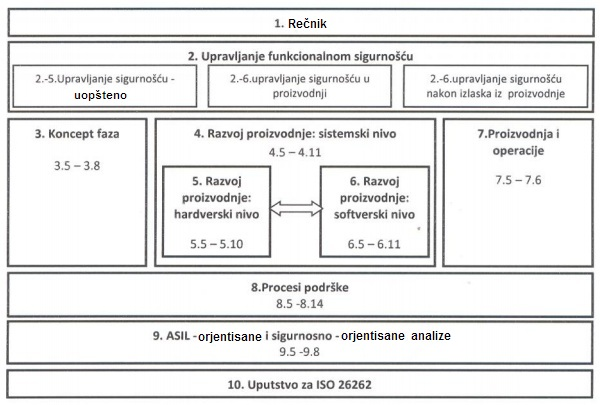
\includegraphics[scale=0.5]{primenastandarda.jpg}
\end{center}
\caption{Struktura serije standarda ISO 26262 sa područjem primene njegovih delova}
\label{fig:primenastandarda}
\end{figure}

Kratak opis delova standarda \cite{ref37}:
\begin{itemize}
  \item ISO 26262-1 predstavljen na samom vrhu šematskog prikaza specificira pojmove, definicije i skraćenice za aplikaciju koje se koriste u svim ostalim delovima standarda
  \item ISO 26262-2 specificira zahteve za upravljanje funkcionalnom sigurnošću za automobilske aplikacije, uključujući zahteve nezavisne od projekta a koji se tiču organizacija uključenih u projekat (sveobuhvatno upravljanje sigurnošću) i zahteve zavisne od projekta a koji se tiču aktivnosti upravljanja u sigurnosnom ciklusu (upravljanje tokom koncept faze i razvoja proizvoda, i nakon puštanja u rad za proizvodnju)
  \item ISO 26262-3 specificira zahteve za koncept fazu automobilskih aplikacija, uključujući: definiciju stavki (eng. item), iniciranje sigurnosnog ciklusa, analize opasnosti i procene rizika i koncept funkcionalne sigurnosti
  \item ISO 26262-4 specificira zahteve za razvoj proizvoda na sistemskom nivou, uključujući: uslovi za pokretanje razvoja proizvoda, specifikacija tehničkih sigurnosnih zahteva, tehnički koncept sigurnosti, dizajn sistema, integracija stavki i testiranje, sigurnosna provera, procena funkcionalne sigurnosti i puštanje proizvoda u rad
 \item ISO 26262-5 specificira zahteve za razvoj proizvoda na hardverskom nivou, uključujući: uslovi za pokretanje razvoja proizvoda na hardverskom nivou, specifikacija hardverskih sigurnosnih zahteva, dizajn hardvera, podaci hardverskog nivoa i procena kršenja bezbednosne granice usled slučajnih grešaka hardvera, njegova integracija i testiranje
 \item ISO 26262-6 specificira zahteve za razvoj proizvoda na softverskom nivou, uključujući: uslovi za pokretanje razvoja proizvoda na softverskom nivou, specifikacija softverskih sigurnosnih zahteva, dizajn softverske arhitekture, dizajn softverskih jedinica i njihovih implentacija, testiranje softverskih jedinica, softverska integracija i testiranje i provera softverskih sigurnosnih zahteva
 \item ISO 26262-7 specificira zahteve za proizvodnju, rad, usluge i razgradnju
 \item ISO 26262-8 specificira zahteve za prateće procese
 \item ISO 26262-9 specificira zahteve za ASIL (eng. Automotive Safety Integrity Level) orjentisanu i sigurnosno orjentisanu analizu
 \item ISO 26262-10 predstavlja sveobuhvatni prikaz ISO 26262 standarda, pruža dodatna obrazloženja u cilju razumevanja drugih delova ISO 26262
\end{itemize}
\bigbreak

\section{Zaključak i budući rad}
\label{sec:zakljucak}

U ovom radu dali smo pregled nekih izazova u testiranju softvera za automobile. Fokusirali smo se na scenarije testiranja crne kutije, pošto izvorni kod često nije dostupan u scenariju GEM-dobavljača u automobilskom domenu. Nakon opšteg procesa testiranja, predstavili smo šest pristupa za poboljšanje efikasnosti testiranja s obzirom na ograničenja razvoja softvera za automobile. Neki od predloženih koncepata su već ostvarivi,
na primer, sistematski opis slučaja testa. Drugi trebaju neke buduće radnje da bi bili od praktične upotrebe, npr., Pristupi u mašinskom učenju u testiranju u crnoj kutiji.
\bigbreak

\begin{thebibliography}{9}
\bibitem{ref1} 
F. Saglietti, “Testing for dependable embedded software,” in 36th EUROMICRO Conference on Software Engineering and Advanced Applications (SEAA). IEEE, 2010, pp. 409–416.
 
\bibitem{ref2} 
K. Grimm, “Software technology in an automotive company: major challenges,” in Proceedings of the 25th International Conference on Software Engineering. IEEE Computer Society, 2003, pp. 498–503.
 
\bibitem{ref3} 
Umar Zakir Abdul, Hamid; et al. (2017). "Autonomous Emergency Braking System with Potential Field Risk Assessment for Frontal Collision Mitigation". 2017 IEEE Conference on Systems, Process and Control (ICSPC). Retrieved 14 March 2018.

\bibitem{ref4}
B. Katumba and E. Knauss, “Agile development in automotive software development: Challenges and opportunities,” in Product-Focused Software Process Improvement. Springer, 2014, pp. 33–47. 

\bibitem{ref5}
F. Fabbrini, M. Fusani, G. Lami, and E. Sivera, “Software engineering in the European automotive industry: Achievements and challenges,” in 32nd Annual IEEE Computer Society International Conference on Computers, Software and Applications(COMPSAC), 2008, pp. 1039–1044.

\bibitem{ref6}
M. Broy, “Automotive software and systems engineering,” in Proceedings of the 3rd ACM and IEEE International Conference on Formal Methods and Models for Co-Design(MEMOCODE), 2005, pp. 143–149. 

\bibitem{ref7}
M. Broy, I. H. Kruger, A. Pretschner, and C. Salzmann, “Engineering automotive software,” Proceedings of IEEE, vol. 95, no. 2, pp. 356–373, 2007. 

\bibitem{ref8}
J. S. Her, S. W. Choi, J. S. Bae, S. D. Kim, and D. W. Cheun, “A component-based process for developing automotive ecu software,” in Product-Focused Software Process Improvement. Springer, 2007, pp. 358– 373.

\bibitem{ref9}
F. Franco, M. Mauro, S. Stevan, A. B. Lugli, and W. Torres, “Modelbased functional safety for the embedded software of automobile power window system,” in 11th IEEE/IAS International Conference on Industry Applications (INDUSCON), 2014, pp. 1–8. 

\bibitem{ref10}
M. Conrad, "Verification and validation according to ISO 26262: A workflow to facilitate the development of high-integrity software" Proceedings to 6th European Congress on Embedded Real Time Software and Systems (ERTS2), 2012. 

\bibitem{ref11}
S. S. Barhate, "Effective test strategy for testing automotive software"in International Conference on Industrial Instrumentation and Control (ICIC). IEEE, 2015, pp. 645–649. 

\bibitem{ref12}
R. Awedikian and B. Yannou, "A practical model-based statistical approach for generating functional test cases: application in the automotive industry Software Testing, Verification and Reliability, vol. 24, no. 2, pp. 85–123, 2014.

\bibitem{ref13}
A. Kasoju, K. Petersen, and M. V. Mäntylä, “Analyzing an automotive testing process with evidence-based software engineering,” Information and Software Technology, vol. 55, no. 7, pp. 1237–1259, 2013. 

\bibitem{ref14}
D. Sundmark, K. Petersen, and S. Larsson, "An exploratory case study of testing in an automotive electrical system release process" in 6th IEEE International Symposium on Industrial Embedded Systems (SIES). IEEE, 2011, pp. 166–175. 

\bibitem{ref15}
A. M. Pérez and S. Kaiser, “Top-down reuse for multi-level testing,” in 17th IEEEInternationalConferenceandWorkshopsonEngineeringofComputer Based Systems (ECBS), 2010, pp. 150–159. 

\bibitem{ref16}
J. Kasurinen, O. Taipale, and K. Smolander. Software Test Automation in Practice: Empirical Observations. Advances in Software Engineering, 2010: 571-579, 2010. 

\bibitem{ref17}
S. Lity, R. Lachmann, M. Lochau, and I. Schaefer. Delta-oriented Software Product Line Test Models - The Body Comfort System Case Study. Technical report, TU Braunschweig, 2013.

\bibitem{ref18}
M. Lochau, S. Lity, R Lachmann, I. Schaefer, and U. Goltz. Delta-oriented model based integration testing of large-scale systems. The Journal of Systems and Software, 91: 63-84, 2014.

\bibitem{ref19}
L. Zhang, D.Han, L.Zhang, G.Rothermel, and H. Mei. Bridging the Gap between the Total and Additional Test-Case Prioritization Strategies. In International Conferenceon Software Engineering, ICSE 2013, 2013

\bibitem{ref20}
R. Lachmann and I. Schaefer. Herausforderungen beim Testen von Fahrerassistenzsystemen. In 11. Workshop Automotive Software Engineering (ASE), 2013.

\bibitem{ref21}
G. Rothermel, R. H. Untch, C. Chu, and M. J. Harrold. Prioritizing Test Cases For Regression Testing. IEEE Transactions on software engineering, Vol.27 No.10:929-948,2001.

\bibitem{ref22}
C. Kaner. What is a good test case? In Software Testing Analysis and Review Conference (STAR) East, 2003.

\bibitem{ref23}
M.Utting and B.Legeard. Practical Model-based Testing. Morgan Kaufmann, 2007.

\bibitem{ref24}
M. A. Sindbu and 1c. Meinkc. ms: An lncnemntal Lemming Algorithm for Finite Automata. CoRR, abs/1206.2691, 2012.

\bibitem{ref25}
H. Raffelt, B. Steffen, and T. Margaria. Dynamic Testing via Automata Learning. In Proceedings of the 3rd International Haifa Verification Conference on Hardware and Software: Verification and Testing, HVC'07, pages 136-152. Springer-Verlag, 2008

\bibitem{ref26}
L.C. Briand. Novel Applications of Machine Learning and Software Testing. In Quality Software, 2008 QSIC '08. The Eighth International Conference on, pages 3-10, Aug 2008.

\bibitem{ref27}
A R. Lenz, A. P020, and S. R. Vergilio. Linking software testing results with a machine learning approach. Engineering Applications of Artificial Intelligence, 266-6): 1631-1640, 2013.

\bibitem{ref28}
F. A. Barros, L. Neves, E. Hori, and D. Torres. The ucsCNL: A Controlled Natural Language for Use Case Specifications. In SEKE, pages 250-253. Knowledge Systems Institute Graduate School, 2011.

\bibitem{ref29}
J. Ferrer, P. M. Kruse, F. Chicano, and E. Alba. Evolutionary Algorithm for Prioritized Pairwise Test Data Generation. In Proceedings of the 14th Annual Conference on Genetic and Evolutionary Computation, GECCO '12, pages 1213-1220. ACM, 2012.

\bibitem{ref30}
C.Strobbe, S.Herramhof, E.Vlachogiannis, and C.A. Velasco. Test Case Description Language (TCDL): Test Case Metadata for Conformance Evaluation. In ICCHP, pages 164-171, 2006.

\bibitem{ref31}
E. Engstrom and P. Runeson. Software product line testing - A systematic mapping study. Information and Software Technology, 53:2-13, 2011.

\bibitem{ref32}
A. Cmyrev and R. ReiBig. Optimierte Varianten- und Anforderungsabdeckung im Test. In Automotive Software Engineering Workshop. 43. GI Jahrestagung, 2013.

\bibitem{ref33}
M.F. Johansen, O.Haugen, and F. Fleurey. An algorithm for generating t-wise covering arrays from large feature models. In SPLC, pages 46-55, 2012.

\bibitem{ref34}
L.C. Briand, Y. Labiche, and Z. Bawar. Using the Machine Learning to Refine Black-Box Test Specifications and Test Suites. In Quality Software, 2008. QSIC'08. The Eighth International Conference, pages 135-144, Aug 2008. 

\bibitem{ref35}
B. Engstrom, P. Runeson, and M. Skoglund. A systematic review on regression test selection techniques. Information and Software Technology, 52: 14-30, 2010.

\bibitem{ref36}
Sabira S. Salihović, Suada F. Dacić, Azra A. Ferizović, Funkcionalna sigurnost cestovnih vozila prema seriji standarda ISO 26262, 2015.

\bibitem{ref37}
International Organization for Standardization (ISO), ISO 26262-Part 1 - Part 9: Road vehicles - Functional safety, 2011.

\bibitem{ref38}
Distributed Development of Automotive Real-time Systems based on Function-triggered Timing Constraints, Oliver Scheickl, Christoph Ainhauser, Michael Rudorfer BMW Car IT, Munich, Germany  
\end{thebibliography}
\end{document} 
